\documentclass[12pt]{article}

\usepackage{fullpage}
\usepackage{multicol,multirow}
\usepackage{tabularx}
\usepackage{listings}
\usepackage{pgfplots}
\usepackage[utf8]{inputenc}
\usepackage[russian]{babel}
\usepackage{pgfplots}
\usepackage{tikz}

% Оригиналный шаблон: http://k806.ru/dalabs/da-report-template-2012.tex

\begin{document}

\section*{Лабораторная работа №9\, по курсу дискрeтного анализа: Графы}

Выполнил студент группы М8О-312Б-22 МАИ \textit{Юрков Евгений}.

\subsection*{Условие}

\textbf{Вариант:} 4

Поиск кратчайшего пути между парой вершин алгоритмом Дейкстры

Задан взвешенный неориентированный граф, состоящий из n вершин и m ребер.
Вершины пронумерованы целыми числами от 1 до n.
Необходимо найти длину кратчайшего пути из вершины с номером start в вершину с номером finish
при помощи алгоритма Дейкстры. Длина пути равна сумме весов ребер на этом пути.
Граф не содержит петель и кратных ребер.

\textbf{Формат ввода:}
В первой строке заданы $1 \leq n \leq 10^5$ и $1 \leq m \leq 10^5$, $1 \leq start \leq n$ и $1 \leq finish \leq n$.
В следующих m строках записаны ребра.
Каждая строка содержит три числа – номера вершин, соединенных ребром, и вес данного ребра. Вес ребра – целое число от 0 до $10^9$.

\textbf{Формат вывода:}
Необходимо вывести одно число – длину кратчайшего пути между указанными вершинами.
Если пути между указанными вершинами не существует, следует вывести строку "No solution" (без кавычек).
\newpage
\subsection*{Метод решения}

Для решения задачи я реализовал алгоритм Дейкстры для нахождения кратчайшего пути во взвешенном графе.
Его смысл состоит в том, что на каждом шаге мы выбираем ту вершину, известный путь до которой является наименьшим среди всех известных.
Далее происходит релаксация рёбер через эту вершину, так подбирается кратчайший путь для последующих вершин.
Чтобы на каждом шагу подбирать вершину с минимальной длиной пути используется очередь с приоритетом.

% \newpage
\subsection*{Описание программы}

Алгоритм Дейкстры реализован в функции 
\texttt{std::vector<int64\_t> dijkstra(
    const std::vector<std::vector<std::pair<int, int64\_t>>>\& graph, int start)},
принимающей на вход взвешенный граф и вершину, от которой следует считать пути.
Эта функция возвращает массив длин путей для каждой вершины (если пути нет, то там будет INF)

%\newpage
\subsection*{Дневник отладки}

Программа не прошла тестирование с первого раза, так как сначала была допущена ошибка в инициализации
очереди с приоритетом. Нужно было указать другой компаратор в параметрах шаблона.

\newpage
\subsection*{Тест производительности}

Алгоритм Дейкстры имеет сложность $O((V + E) \log V)$.
\begin{figure}
    \centering
    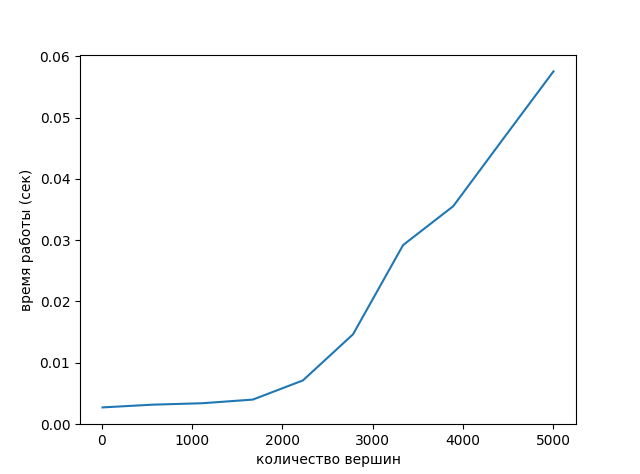
\includegraphics[width=\textwidth]{graph.png}
    \caption{График зависимости времени работы программы от количества вершин в графе}
\end{figure}

% \newpage
\subsection*{Выводы}

Эта работа позволила мне углубиться в основы работы с графами,
их представлением в памяти и реализацией классических алгоритмов.
Основные сложности возникали при организации управления очередью,
чтобы избежать ошибок неверного обновления приоритетов.

Полученные навыки важны для решения задач маршрутизации,
моделирования сетей и анализа взаимосвязей в данных.
Понимание алгоритмов на графах и их оптимизация
может быть применено в таких областях, как транспортные системы,
социальные сети, а также задачи планирования и логистики.
\end{document}